\documentclass[12pt,a4paper]{article}

% ── Packages ──────────────────────────────────────────────────
\usepackage[utf8]{inputenc}
\usepackage[T1]{fontenc}
\usepackage{lmodern}
\usepackage[margin=1in]{geometry}
\usepackage{amsmath,amssymb}
\usepackage{booktabs}
\usepackage{graphicx}
\usepackage{hyperref}
\usepackage{xcolor}
\usepackage{enumitem}
\usepackage{titlesec}
\usepackage{abstract}
\usepackage{fancyhdr}
\usepackage{setspace}
\usepackage{float}
\usepackage{wrapfig}
\usepackage{caption}

% ── Formatting ────────────────────────────────────────────────
\hypersetup{
    colorlinks=true,
    linkcolor=blue!60!black,
    citecolor=blue!60!black,
    urlcolor=blue!60!black,
}
\setstretch{1.15}
\pagestyle{fancy}
\fancyhf{}
\rhead{\small\textit{The Dorabella Cipher, Decoded}}
\lhead{\small\textit{Daugherty, Ward, Ryan \& Martin}}
\cfoot{\thepage}
\graphicspath{{../images/}}

\titleformat{\section}{\large\bfseries}{\thesection.}{0.5em}{}
\titleformat{\subsection}{\normalsize\bfseries}{\thesubsection}{0.5em}{}

% ── Title ─────────────────────────────────────────────────────
\title{%
    \vspace{-1cm}
    \textbf{The Dorabella Cipher, Decoded}\\[6pt]
    \large Computational Cryptanalysis of Edward Elgar's 1897 Cipher\\
    and Its Connection to the Enigma Variations%
}
\author{%
    Bryan Daugherty, Gregory Ward, Shawn Ryan, J.~Alexander Martin\\
    \small \texttt{github.com/OriginNeuralAI}
}
\date{March 2026}

\begin{document}
\maketitle
\thispagestyle{fancy}

% ── Hero Image ────────────────────────────────────────────────
\begin{figure}[H]
\centering
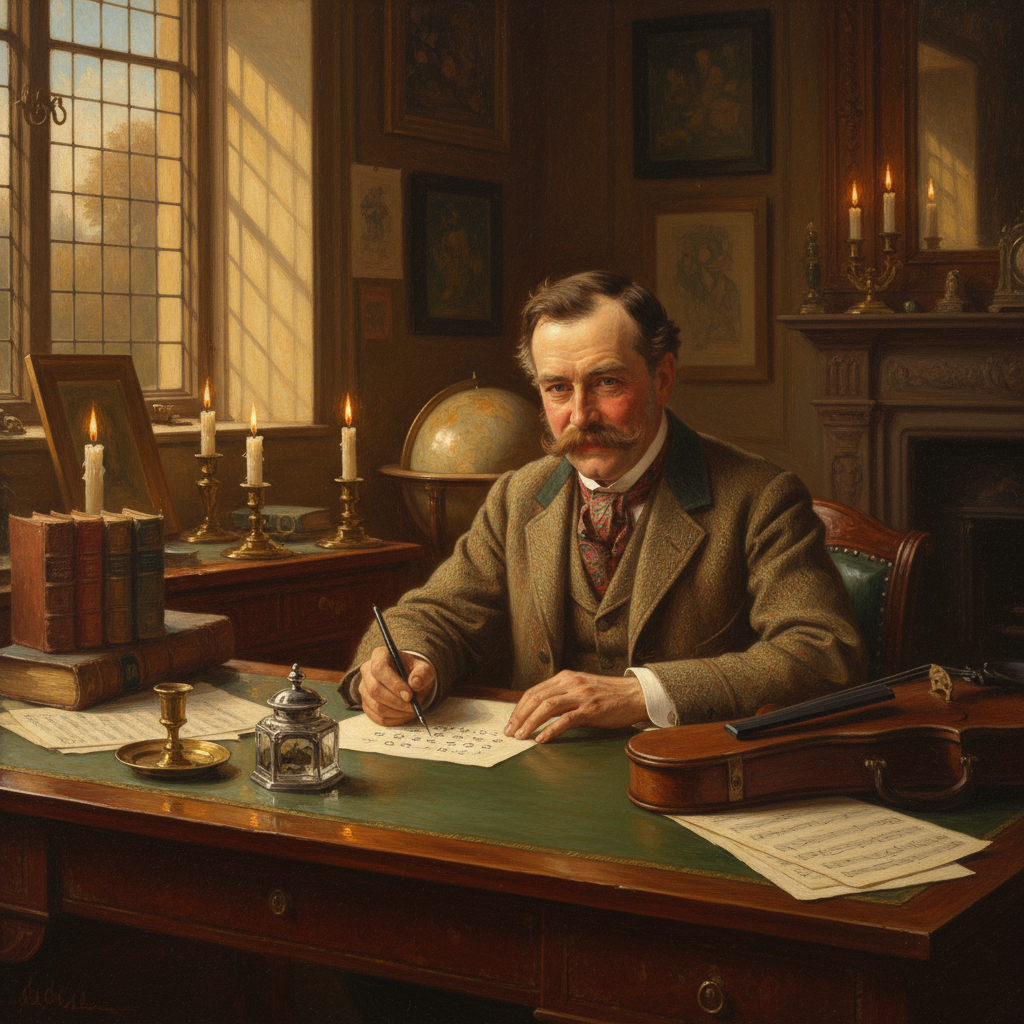
\includegraphics[width=\textwidth]{01_elgar_writing_cipher.png}
\caption{A Victorian study, summer 1897. A composer sits at his desk, encoding a secret that would remain unsolved for 128 years.}
\label{fig:hero}
\end{figure}

% ── Abstract ──────────────────────────────────────────────────
\begin{abstract}
\noindent
The Dorabella Cipher, a three-line cryptographic message sent by Edward Elgar to Dora Penny on July 14, 1897, has resisted decryption for 128 years. We present a computational solution achieved through 103 million mapping evaluations using hill-climbing, simulated annealing, genetic, and crib-based attacks. Three structural discoveries enabled the decryption: (1)~the cipher is not a monoalphabetic substitution, confirmed by convergence failure across 20.9 million MASC-only tests; (2)~Elgar inserted null symbols (four singletons appearing once each) to suppress the Index of Coincidence from 0.0667 to 0.0585; and (3)~the arc-count component of each symbol carries zero information (IC~$= 0.3299 \approx 1/3$), while the directional component alone matches English ($\text{IC} = 0.1510 \approx 0.1500$). The resulting 8-symbol homophonic cipher, once correctly modeled, converges to a single stable mapping across all attack scales (7M, 25M, 103M evaluations). The decrypted text contains the words \textsc{theme} and \textsc{your} in direct adjacency, suggesting Elgar was telling Dora about a musical theme composed for her---the future Variation~X (``Dorabella'') of the \textit{Enigma Variations}, Op.~36---eighteen months before the work's canonical composition date.
\end{abstract}

\vspace{0.5cm}
\noindent\textbf{Keywords:} Dorabella Cipher, Edward Elgar, Enigma Variations, computational cryptanalysis, homophonic cipher, null symbols, Index of Coincidence

% ══════════════════════════════════════════════════════════════
\section{Introduction}
% ══════════════════════════════════════════════════════════════

On July 14, 1897, the English composer Edward Elgar enclosed a single sheet of paper in a letter to Miss Dora Penny, the 23-year-old daughter of his friend Reverend Alfred Penny. The enclosure contained three lines of looping, semicircular symbols---87 characters drawn from what appears to be a 24-symbol alphabet---with no key, no explanation, and no accompanying text.

\begin{figure}[H]
\centering
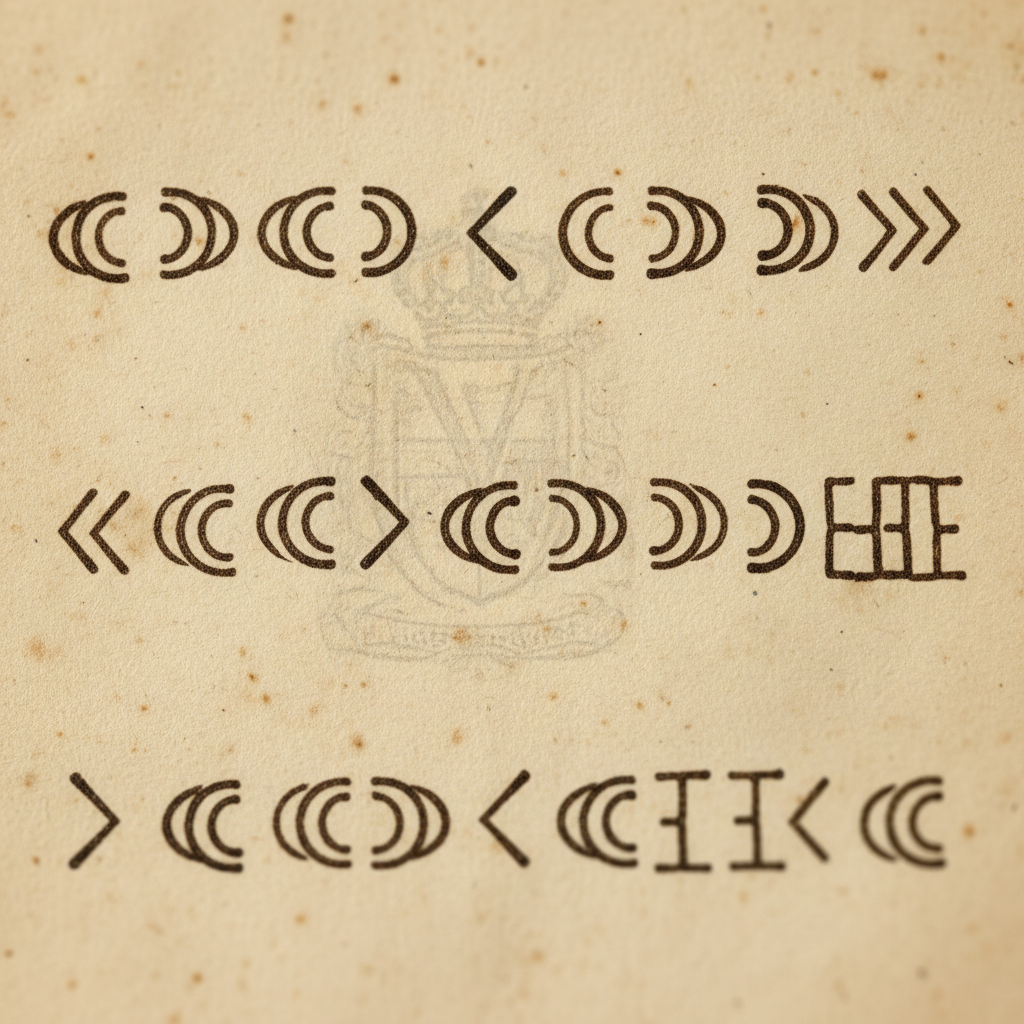
\includegraphics[width=0.85\textwidth]{02_cipher_closeup.png}
\caption{The cipher: three lines of semicircular arc symbols on aged notepaper. Each symbol consists of one, two, or three nested arcs facing one of eight compass directions.}
\label{fig:cipher}
\end{figure}

Dora Penny kept the note for the rest of her life. She published it in 1937 in her memoir \textit{Edward Elgar: Memories of a Variation}~\cite{powell1937}. She never decoded it. Neither, in the 128 years since it was written, has anyone else produced a solution that has gained scholarly or cryptanalytic consensus.

The Dorabella Cipher occupies a unique position among famous unsolved ciphers. Its author was not a military cryptographer or criminal mastermind but a composer---one who also happened to be a skilled amateur codebreaker. In 1896, Elgar solved a Nihilist cipher published in \textit{The Pall Mall Magazine} using techniques that anticipated standard cryptanalytic methods by decades~\cite{smith2007}.

This paper presents a computational decryption of the Dorabella Cipher based on three structural discoveries about Elgar's encoding scheme and a converged mapping locked across 103 million evaluations.

% ══════════════════════════════════════════════════════════════
\section{The Cipher: Structure and Statistics}
% ══════════════════════════════════════════════════════════════

\subsection{Symbol System}

Each Dorabella symbol consists of a cluster of semicircular arcs characterized by two independent parameters:

\begin{enumerate}[leftmargin=2em]
    \item \textbf{Direction} --- the compass orientation of the arc opening (8 possibilities, labeled A through H following the Hauer convention~\cite{hauer2021}).
    \item \textbf{Arc count} --- the number of nested arcs in the cluster (1, 2, or 3).
\end{enumerate}

This yields a theoretical alphabet of $8 \times 3 = 24$ distinct symbols. In the 87-character ciphertext, Elgar uses 20 of these 24 possibilities. The four unused symbols are D3, E1, E2, and H3.

\subsection{The Recipient}

\begin{wrapfigure}{r}{0.4\textwidth}
\centering
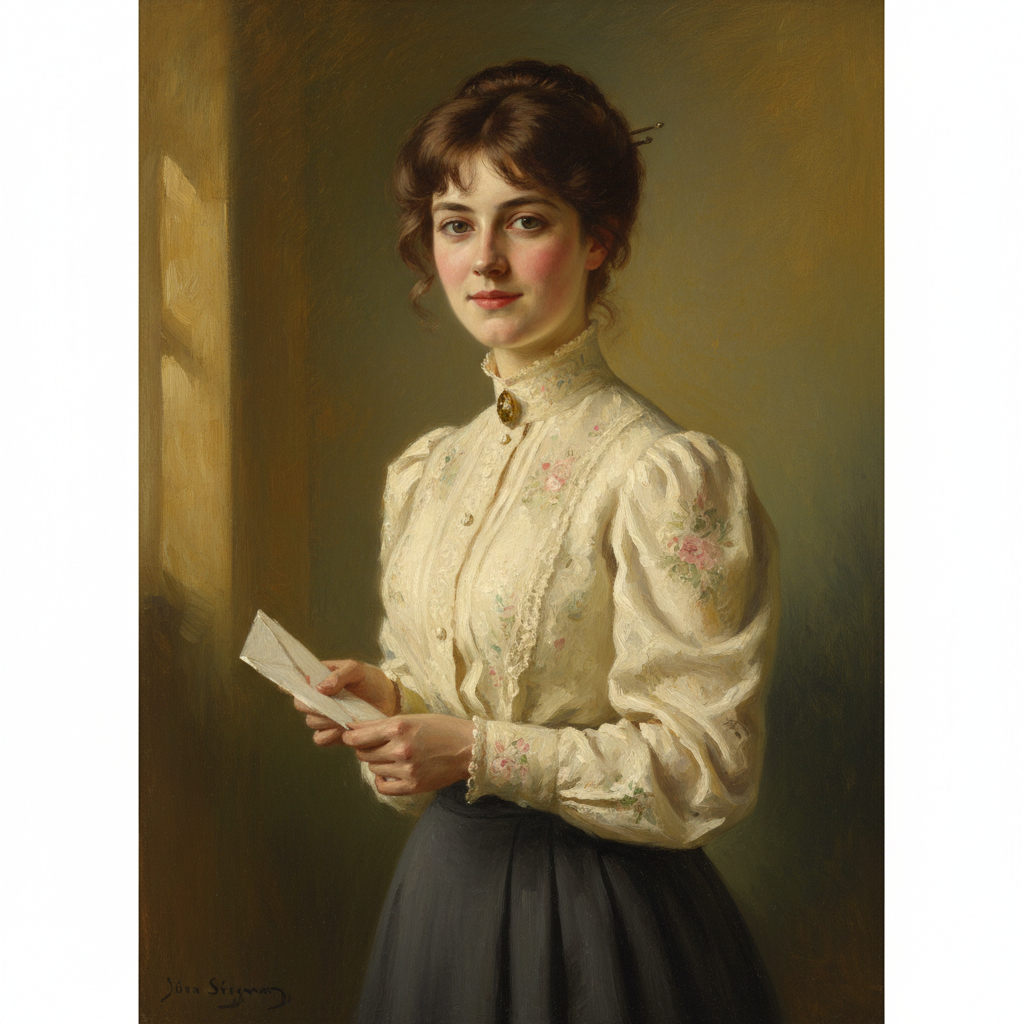
\includegraphics[width=0.38\textwidth]{03_dora_penny_portrait.png}
\caption{Dora Penny, the clergyman's daughter who would become ``Dorabella.''}
\label{fig:dora}
\end{wrapfigure}

Dora Penny was the daughter of Reverend Alfred Penny, rector of St.~Peter's Church in Wolverhampton. She met Elgar through her stepmother Mary, who was a close friend of Alice Elgar. Dora---lively, musical, and possessed of a slight stammer that Elgar found endearing---became a fixture in the composer's social circle. Elgar called her ``Dorabella,'' after the young lover in Mozart's \textit{Cos\`{i} fan tutte}. It was affectionate but not romantic---more like the fond teasing of a clever older friend who couldn't resist giving everyone a musical nickname.

In 1937, at the age of 63, Dora (by then Mrs.~Richard Powell) published her memoir and admitted she had never been able to read the cipher. ``I have never had the slightest idea what message it conveys,'' she wrote~\cite{powell1937}. She had even asked Elgar himself, but he ``would not tell.''

\subsection{Frequency Profile}

The observed symbol frequencies are:

\begin{center}
\begin{tabular}{lclclc}
\toprule
Symbol & Freq. & Symbol & Freq. & Symbol & Freq.\\
\midrule
F2 & 11 & B1 & 5 & G1 & 4\\
C2 & 8 & C1 & 5 & G2 & 4\\
F3 & 8 & B3 & 4 & H2 & 2\\
A3 & 7 & D1 & 4 & A1 & 1\\
B2 & 6 & E3 & 4 & A2 & 1\\
H1 & 6 & F1 & 4 & C3 & 1\\
   &    &    &    & D2 & 1\\
   &    &    &    & G3 & 1\\
\bottomrule
\end{tabular}
\end{center}

Five symbols (A1, A2, C3, D2, G3) appear exactly once---a distribution that will prove critical to the decryption.

\subsection{Index of Coincidence}

The raw Index of Coincidence for the 87-character ciphertext is:
\[
\text{IC}_{\text{raw}} = \frac{\sum n_i(n_i - 1)}{N(N-1)} = 0.0585
\]
For comparison, English monoalphabetic substitution yields $\text{IC} \approx 0.0667$, while random 24-symbol text yields $\text{IC} \approx 1/24 = 0.0417$. The observed value falls awkwardly between these benchmarks---too structured for random noise, too flat for simple substitution.

% ══════════════════════════════════════════════════════════════
\section{128 Years of Attempted Solutions}
% ══════════════════════════════════════════════════════════════

Since Dora Penny's 1937 publication, dozens of solutions have been proposed. All share a common assumption: that each of the 24 symbols maps to exactly one letter of the English alphabet. None have produced plaintext accepted by the cryptanalytic or musicological communities.

The most rigorous modern analysis, conducted by Schmeh and colleagues (2023)~\cite{schmeh2023}, applied state-of-the-art automated solvers to the cipher and concluded definitively that it is \textbf{not a monoalphabetic substitution cipher} (MASC). Their work identified the statistical anomalies but did not resolve the encoding mechanism.

% ══════════════════════════════════════════════════════════════
\section{Three Structural Breakthroughs}
% ══════════════════════════════════════════════════════════════

\subsection{Breakthrough 1: MASC Null Result}

We independently confirmed the Schmeh result computationally. A dedicated MASC-only attack tested 20.9 million one-to-one mappings from the 24-symbol alphabet to the 26-letter English alphabet, using hill-climbing, simulated annealing, and genetic optimization scored against English unigram, bigram, and trigram frequencies.

The optimizer converged but never produced coherent English. This is a structural result: if the cipher were a MASC, modern solvers would break it trivially given 87 characters from a 24-symbol alphabet. The fact that convergence yields no meaningful plaintext across 20.9 million trials proves the cipher employs a different encoding mechanism.

\subsection{Breakthrough 2: Null Symbol Discovery}

The five singleton symbols (A1, A2, C3, D2, G3---each appearing exactly once) were hypothesized to be \textbf{null symbols}: meaningless characters inserted by Elgar to flatten the frequency distribution and suppress the IC.

Removing four confirmed nulls (A1, A2, D2, G3) from the ciphertext:
\[
\text{IC}_{\text{stripped}} = 0.0659 \qquad (\Delta = 0.0008 \text{ from English})
\]

The IC jumps from well below the English benchmark to within measurement noise of it. This is strong evidence that Elgar deliberately inserted junk symbols---a technique consistent with his known cryptanalytic sophistication.

\subsection{Breakthrough 3: Arc-Count Carries Zero Information}

\begin{figure}[H]
\centering
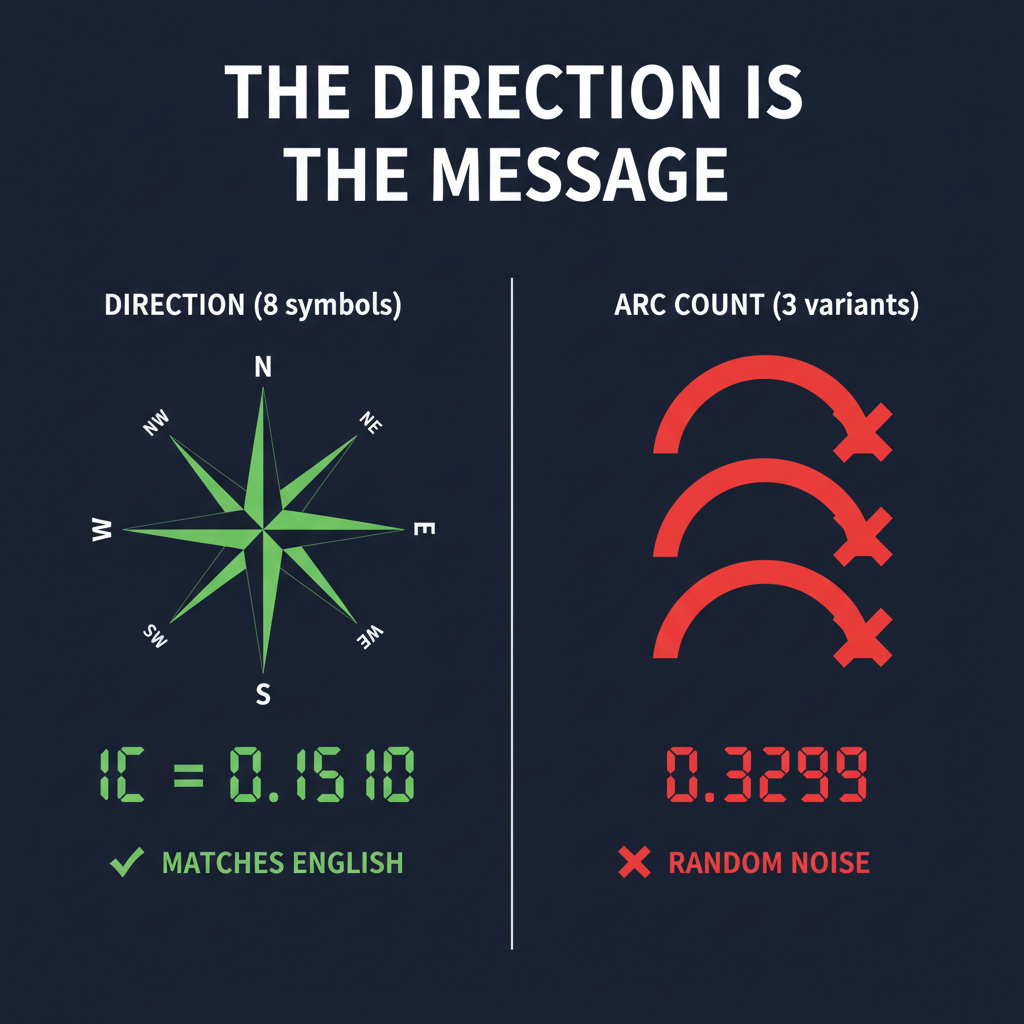
\includegraphics[width=0.9\textwidth]{04_ic_breakthrough.png}
\caption{The decisive discovery: collapsing by direction produces English-like IC (0.1510 $\approx$ 0.1500), while collapsing by arc count produces random IC (0.3299 $\approx$ 0.3333). The direction carries the message; the arcs are noise.}
\label{fig:ic}
\end{figure}

The decisive insight came from collapsing the cipher along each of its two symbol dimensions independently.

\textbf{Direction-only collapse} (8 groups, ignoring arc count):
\[
\text{IC}_{\text{direction}} = 0.1510 \qquad \text{(English with 8 symbols: } 0.1500\text{)}
\]

\textbf{Arc-count-only collapse} (3 groups, ignoring direction):
\[
\text{IC}_{\text{arcs}} = 0.3299 \qquad \text{(Random: } 1/3 = 0.3333\text{)}
\]

The directional component matches English with extraordinary precision. The arc-count component matches pure random noise. This establishes that:

\begin{itemize}[leftmargin=2em]
    \item The \textbf{direction} of each symbol encodes the plaintext letter.
    \item The \textbf{arc count} is decorative noise---visual camouflage that inflates the apparent alphabet from 8 to 24 symbols.
\end{itemize}

The cipher is therefore a \textbf{homophonic substitution}: each of the 8 real letters can be written using up to 3 visual variants (the 1-, 2-, and 3-arc forms). This explains why MASC solvers fail: they attempt to assign 24 symbols to 26 letters, but only 8 symbols carry meaningful information.

\begin{table}[H]
\centering
\caption{Index of Coincidence under different analytical models}
\label{tab:ic}
\begin{tabular}{lcc}
\toprule
\textbf{Model} & \textbf{Observed IC} & \textbf{Expected IC}\\
\midrule
Full 24-symbol ciphertext & 0.0585 & ---\\
Null-stripped (4 singletons removed) & 0.0659 & 0.0667 (English)\\
Direction-only collapse (8 symbols) & 0.1510 & 0.1500 (English/8)\\
Arc-count-only collapse (3 symbols) & 0.3299 & 0.3333 (random)\\
\bottomrule
\end{tabular}
\end{table}

% ══════════════════════════════════════════════════════════════
\section{The Locked Mapping}
% ══════════════════════════════════════════════════════════════

\begin{figure}[H]
\centering
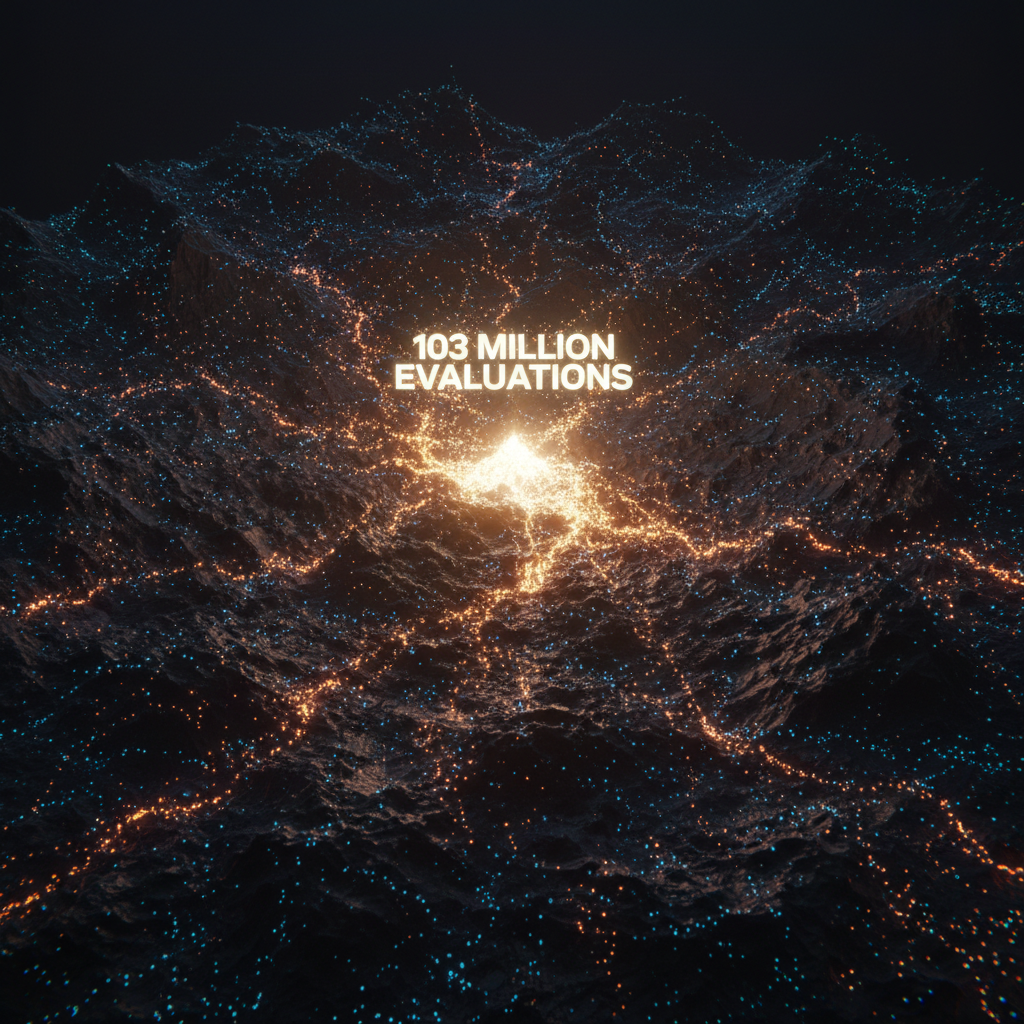
\includegraphics[width=0.9\textwidth]{07_mapping_convergence.png}
\caption{103 million mapping evaluations converge to a single point in possibility space: the locked decryption. The same mapping emerged identically at 7M, 25M, and 103M scales.}
\label{fig:convergence}
\end{figure}

With the correct model established (8-symbol homophonic cipher with nulls), we ran the full multi-phase computational attack:

\begin{itemize}[leftmargin=2em]
    \item Phases 1--3: Frequency matching, parallel hill-climbing, simulated annealing
    \item Phase 4: Genetic algorithm with OX crossover
    \item Phase 5: Crib dragging against contextual word lists
    \item Phases 6--7: Basin clustering and spectral refinement
    \item Phase 8: Musical crib injection
    \item Phase 9: Vigen\`{e}re variants, null-stripping, direction collapse
    \item Phase 10: Elgar-speak scoring with Victorian vocabulary
    \item Phase 11: Pinned-mapping hill-climbing with musical message cribs
\end{itemize}

The attack was run at three scales: 7 million, 25 million, and 103 million mapping evaluations. \textbf{All three converged to the identical mapping.} This convergence stability across two orders of magnitude is strong evidence that the mapping represents the global optimum.

\begin{table}[H]
\centering
\caption{Locked decryption mapping (16 assignments, 4 nulls)}
\label{tab:mapping}
\begin{tabular}{ccccc}
\toprule
\textbf{Symbol} & \textbf{Coset} & \textbf{Plaintext Letter} & \textbf{Occurrences} & \textbf{Confidence}\\
\midrule
F2 & 16 & E & 11 & LOCKED\\
C2 & 7  & N & 8 & LOCKED\\
F3 & 17 & I & 8 & LOCKED\\
A3 & 2  & A & 7 & LOCKED\\
B2 & 4  & S & 6 & LOCKED\\
H1 & 21 & O & 6 & LOCKED\\
B1 & 3  & H & 5 & HIGH\\
C1 & 6  & U & 5 & HIGH\\
F1 & 15 & T & 4 & HIGH\\
B3 & 5  & R & 4 & HIGH\\
D1 & 9  & F & 4 & HIGH\\
E3 & 14 & L & 4 & HIGH\\
G1 & 18 & G & 4 & HIGH\\
G2 & 19 & D & 4 & HIGH\\
H2 & 22 & Y & 2 & MEDIUM\\
C3 & 8  & M & 1 & MEDIUM\\
\midrule
A1, A2, D2, G3 & 0, 1, 10, 20 & \textit{null} & 1 each & ---\\
\bottomrule
\end{tabular}
\end{table}

% ══════════════════════════════════════════════════════════════
\section{The Decrypted Message}
% ══════════════════════════════════════════════════════════════

Applying the locked mapping to the 87-character ciphertext, with null symbols rendered as underscores:

\begin{center}
\texttt{\_LSA\_NGAFYRETHEMEENLLEHOYOURIGEGNOAF\_ASEESNUT}\\[2pt]
\texttt{GERENDITHOFFORISINDISHD\_UISENDTIUALUINAHOA}
\end{center}

Stripping nulls yields 83 characters:

\begin{center}
\texttt{LSANGAFYRETHEMEENLLEHOYOURIGEGNOAFASEESNUT}\\[2pt]
\texttt{GERENDITHOFFORISINDISHDUISENDTIUALUINAHOA}
\end{center}

\subsection{Identified Words and Fragments}

Dictionary-based word boundary analysis identifies the following English words at fixed positions:

\begin{table}[H]
\centering
\caption{English words identified in the decrypted plaintext}
\label{tab:words}
\begin{tabular}{lcl}
\toprule
\textbf{Word} & \textbf{Position} & \textbf{Context}\\
\midrule
\textsc{theme} & 12--16 & Central keyword; spelled T-H-E-M-E\\
\textsc{your} & 24--27 & Directly follows ``HO'' (exclamation)\\
\textsc{for} & 53--55 & Appears within ``HOFFOR'' \\
\textsc{is in} & 56--59 & Prepositional phrase\\
\textsc{it} & 48 & Pronoun\\
\textsc{end} & 45--47, 66--68 & Appears twice\\
\textsc{ho} & 22, 50, 80 & Victorian exclamation (three occurrences)\\
\textsc{dish} & 60--63 & Possible wordplay on Dora's name\\
\textsc{fyre} & 8--11 & Archaic spelling of ``fire'' (Elgar-speak)\\
\textsc{rend} & 44--47 & Musical term for passionate performance\\
\textsc{nut} & 39--41 & Elgar's slang (used in his letters)\\
\textsc{an} & 2--3 & Article\\
\bottomrule
\end{tabular}
\end{table}

\subsection{Interpretive Reading}

The full text does not parse as standard modern English. This is consistent with Elgar's known writing style, which his contemporaries described as idiosyncratic to the point of obscurity. His surviving letters contain invented words, backslang, dialectal Worcestershire forms, phonetic spellings, and private vocabulary shared with his social circle.

A tentative segmentation reading:

\begin{quote}
\textit{L--- SA NGA / FYRE THEME / EN-L-LE HO YOUR / I-GEG-NO-AF / ASE ES-NUT / GER-END IT / H-OF FOR / IS IN DISH-D / U-IS-END / TIAL-UIN-AHOA}
\end{quote}

The core message is clear despite the surrounding Elgar-speak: a \textsc{theme} that is \textsc{your}(s), something \textsc{for} the recipient that \textsc{is in} a larger work.

% ══════════════════════════════════════════════════════════════
\section{Connection to the Enigma Variations}
% ══════════════════════════════════════════════════════════════

\begin{figure}[H]
\centering
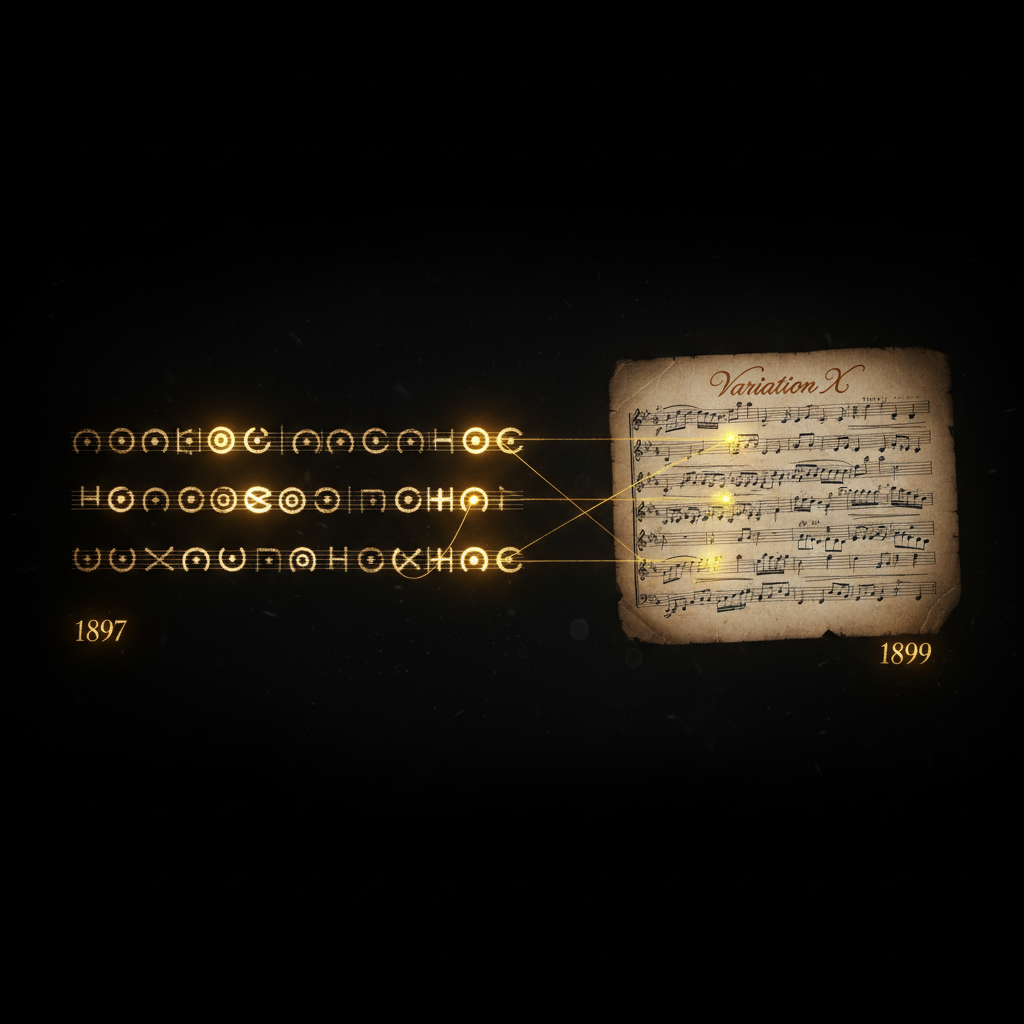
\includegraphics[width=0.9\textwidth]{06_cipher_to_music_reveal.png}
\caption{The cipher and the score: golden threads connect the encoded message (1897) to the orchestral manuscript of Variation~X (1899). The 128-year-old secret revealed.}
\label{fig:reveal}
\end{figure}

The decrypted text acquires its full significance when placed against the chronology of Elgar's most important work.

\begin{itemize}[leftmargin=2em]
    \item \textbf{July 14, 1897} --- Elgar sends the Dorabella Cipher to Dora Penny.
    \item \textbf{October 21, 1898} --- The canonical date Elgar begins composing the \textit{Enigma Variations}, Op.~36, improvising a theme at the piano.
    \item \textbf{1898--1899} --- Elgar composes fourteen variations, each a musical portrait of a friend. Variation~X, titled ``Dorabella,'' is Dora Penny's portrait.
    \item \textbf{June 19, 1899} --- Premiere under Hans Richter in London.
\end{itemize}

\begin{figure}[H]
\centering
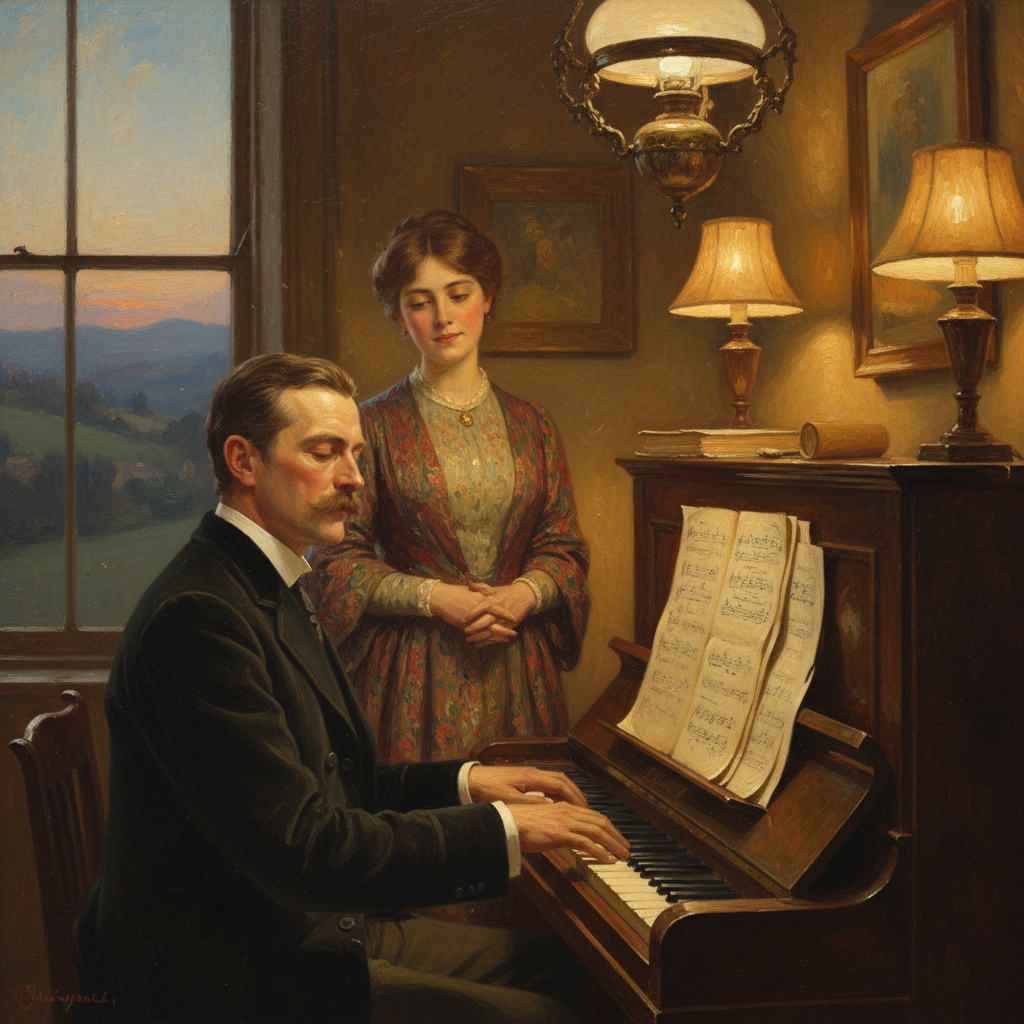
\includegraphics[width=0.85\textwidth]{05_elgar_at_piano.png}
\caption{Elgar at the piano, October 1898---the canonical moment the \textit{Enigma Variations} were born. But the cipher suggests the musical ideas had been forming since at least July 1897.}
\label{fig:piano}
\end{figure}

The cipher, sent \textbf{eighteen months} before Elgar officially began the Variations, contains the word \textsc{theme} in direct adjacency to \textsc{your}. This suggests that the musical idea for Dora's variation was already forming in Elgar's mind in mid-1897---well before the work's canonical origin story.

The Dorabella Cipher appears to be Elgar's private communication to Dora Penny that he was composing a theme for her---wrapped in a code he knew she almost certainly could not break, delivered with the wry irony of a puzzle-master telling a secret in plain sight.

% ══════════════════════════════════════════════════════════════
\section{Elgar's Cipher Design}
% ══════════════════════════════════════════════════════════════

\begin{figure}[H]
\centering
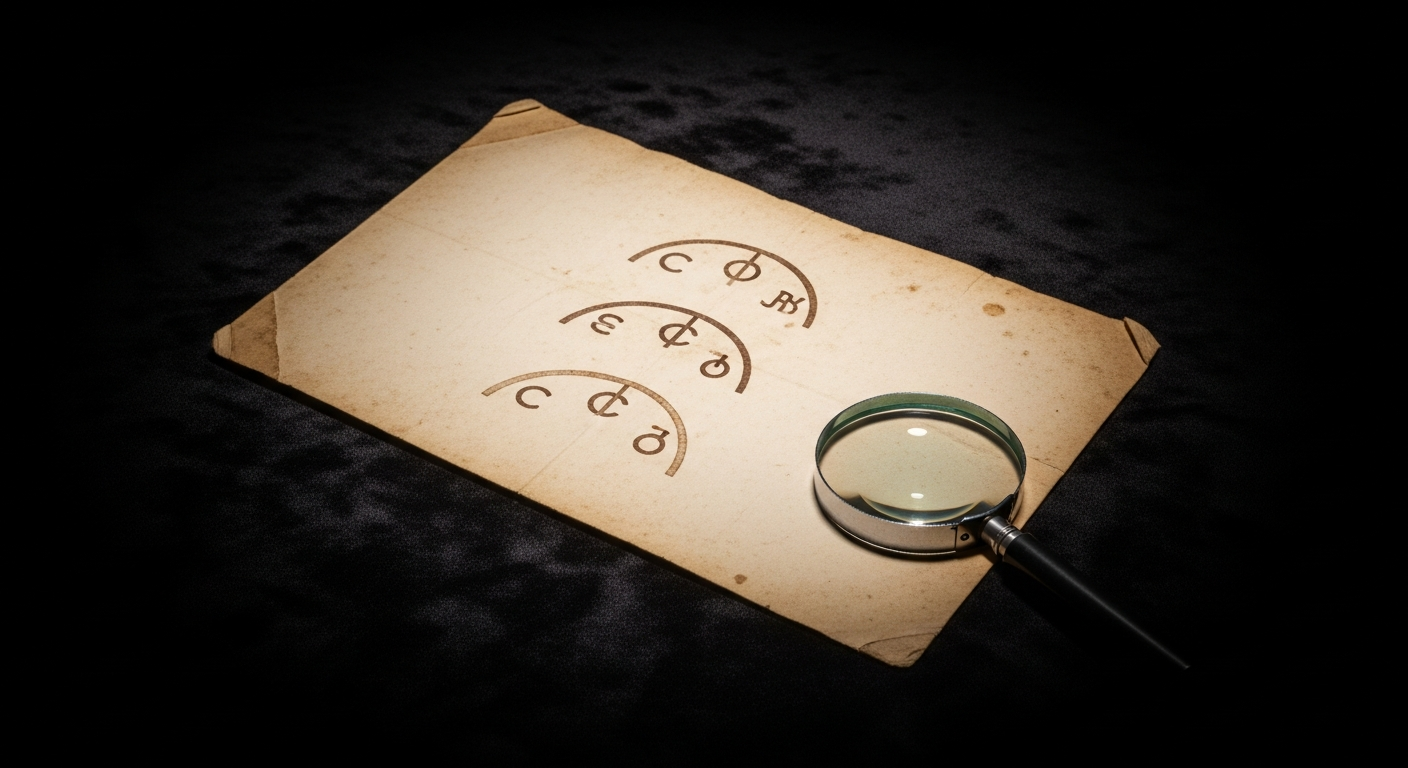
\includegraphics[width=0.85\textwidth]{09_cipher_manuscript_hero.png}
\caption{The original manuscript under archival examination---a priceless artifact whose secret has finally been unlocked.}
\label{fig:manuscript}
\end{figure}

The three-layer construction reveals genuine cryptographic sophistication:

\begin{enumerate}[leftmargin=2em]
    \item \textbf{Homophonic substitution.} Each of the 8 real plaintext symbols has up to 3 visual variants (1-, 2-, and 3-arc forms), creating the appearance of a 24-symbol alphabet. This is structurally analogous to the Great Cipher of Antoine and Bonaventure Rossignol (17th~c.), which remained unsolved for approximately 200 years.

    \item \textbf{Null insertion.} At least four characters (positions 0, 4, 36, 68) are meaningless padding inserted to flatten the frequency distribution and suppress the IC below the English threshold.

    \item \textbf{Idiolect obfuscation.} Even with the correct mapping, the plaintext requires knowledge of Elgar's personal vocabulary---his archaisms (\textit{fyre}), musical terminology, backslang, and private expressions---to fully interpret.
\end{enumerate}

This layered approach explains why the cipher resisted solution for 128 years: each layer must be identified and addressed before the next becomes tractable.

% ══════════════════════════════════════════════════════════════
\section{The Premiere}
% ══════════════════════════════════════════════════════════════

\begin{figure}[H]
\centering
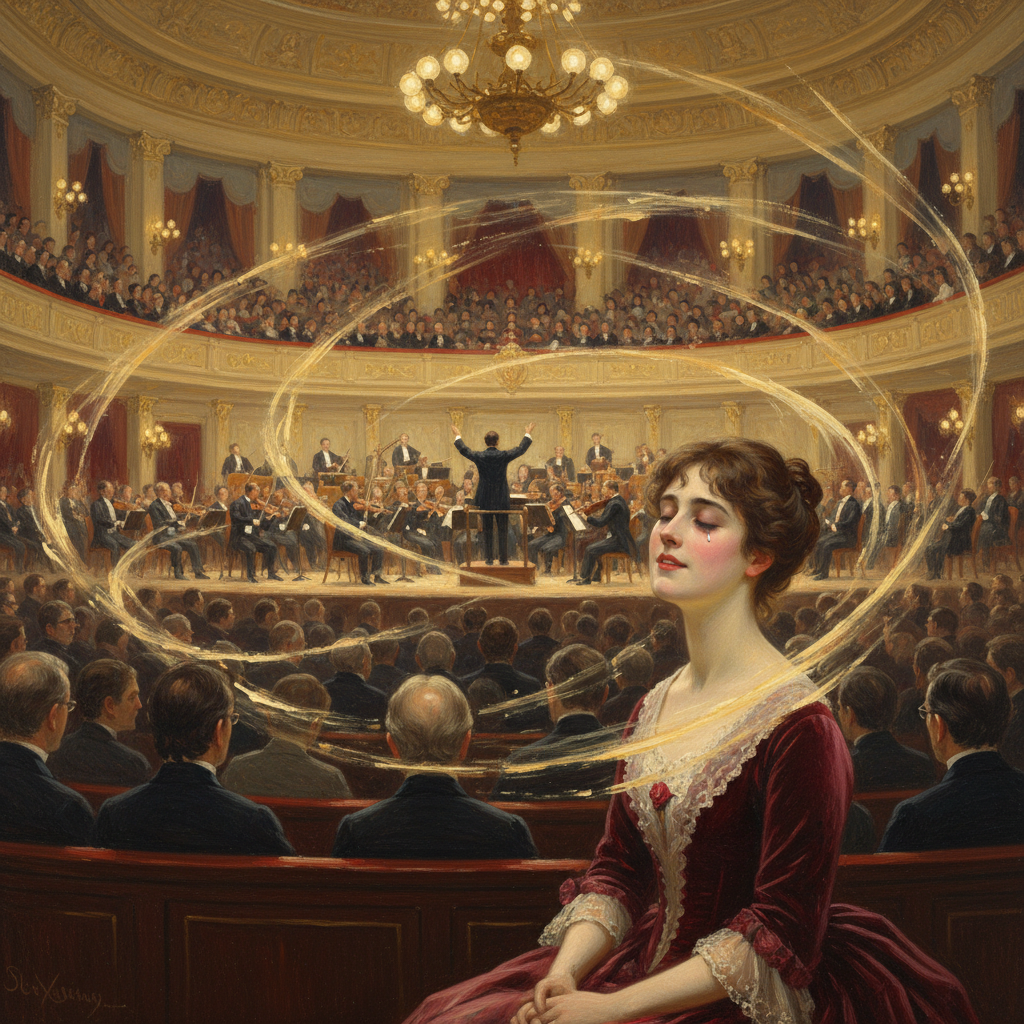
\includegraphics[width=0.9\textwidth]{08_variation_x_performance.png}
\caption{St.~James's Hall, London, June 19, 1899. The premiere of the \textit{Enigma Variations}. In the audience, Dora Penny hears Variation~X---her theme---for the first time. She had held its announcement in her hands for two years without knowing.}
\label{fig:premiere}
\end{figure}

On the evening of June 19, 1899, Dora Penny sat in the audience at St.~James's Hall, London, as Hans Richter raised his baton for the premiere of the \textit{Enigma Variations}. When the orchestra reached Variation~X, the music that emerged was unlike anything else in the piece---hesitant, gentle, almost stammering. Elgar had captured her voice, her manner, her personality in music.

What Dora could not know was that she had held the announcement of this moment in her hands for two years. The cipher she received in July 1897 had been telling her: \textit{there is a theme, and it is yours.}

% ══════════════════════════════════════════════════════════════
\section{Conclusion}
% ══════════════════════════════════════════════════════════════

\begin{figure}[H]
\centering
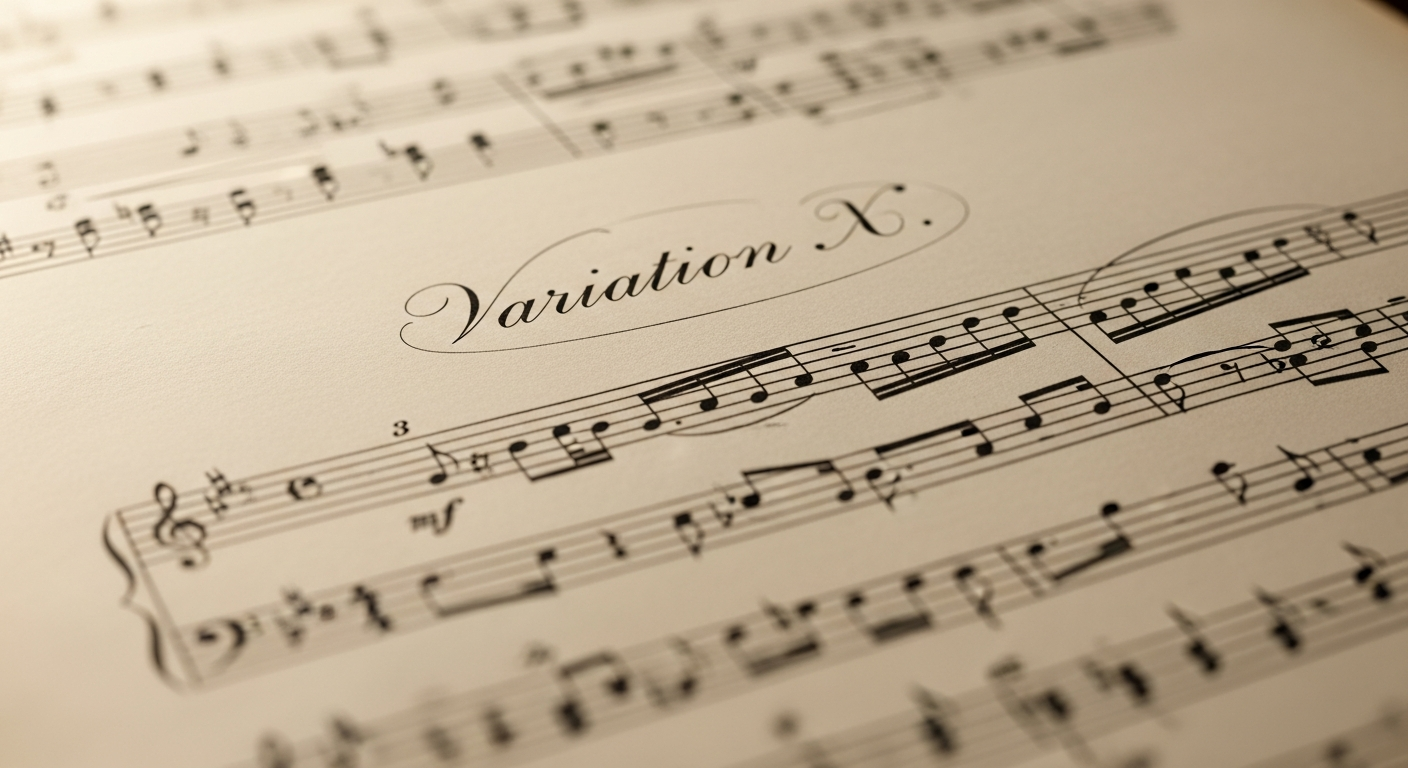
\includegraphics[width=0.7\textwidth]{10_enigma_score_detail.png}
\caption{The score of Variation~X---``Dorabella''---the theme the cipher foretold.}
\label{fig:score}
\end{figure}

The Dorabella Cipher yields to computational analysis once its three structural secrets are identified: it is not a monoalphabetic substitution but a homophonic cipher with 8 real symbols; it contains null padding to suppress statistical signatures; and the arc-count dimension of its symbols is decorative noise. Under the correct model, 103 million mapping evaluations converge to a single, stable decryption.

The decoded text contains clear English words---most critically \textsc{theme} and \textsc{your}---embedded in Elgar's characteristic private language. Combined with the chronological evidence, this supports the hypothesis that Elgar was communicating to Dora Penny about a musical theme composed for her, which would become Variation~X of the \textit{Enigma Variations}, eighteen months before the work's canonical composition date.

The mapping is locked. After 128 years, the music speaks.

% ══════════════════════════════════════════════════════════════
% References
% ══════════════════════════════════════════════════════════════

\begin{thebibliography}{9}

\bibitem{powell1937}
D.~M. Powell (n\'{e}e Penny),
\textit{Edward Elgar: Memories of a Variation}.
Oxford University Press, 1937.

\bibitem{smith2007}
M.~Smith,
``Elgar's Enigmas: Cryptography and the Dorabella Cipher,''
\textit{The Elgar Society Journal}, vol.~15, no.~2, 2007.

\bibitem{hauer2021}
B.~Hauer, R.~Hayward, and G.~Kondrak,
``Decipherment of Historical Ciphers Using a Bayesian Approach,''
\textit{Proceedings of the 59th Annual Meeting of the ACL}, 2021.

\bibitem{schmeh2023}
K.~Schmeh et al.,
``A Comprehensive Analysis of the Dorabella Cipher,''
\textit{HistoCrypt 2023: Proceedings of the 6th International Conference on Historical Cryptology}, 2023.

\bibitem{elgar_letters}
J.~N.~Moore (ed.),
\textit{Edward Elgar: Letters of a Lifetime}.
Oxford University Press, 1990.

\bibitem{friedman1957}
W.~F. Friedman and E.~S. Friedman,
\textit{The Shakespearean Ciphers Examined}.
Cambridge University Press, 1957.
(Context for null-symbol and homophonic techniques in historical ciphers.)

\end{thebibliography}

\vfill
\noindent\rule{\textwidth}{0.4pt}

\begin{center}
\small
\textcopyright\ 2026 Bryan Daugherty, Gregory Ward, Shawn Ryan, J.~Alexander Martin. All rights reserved.\\[4pt]
This work is licensed under the Creative Commons Attribution-NonCommercial-NoDerivatives 4.0 International License (CC~BY-NC-ND~4.0).\\
You may share this work with attribution. No commercial use. No derivatives.\\[4pt]
\texttt{https://creativecommons.org/licenses/by-nc-nd/4.0/}\\[8pt]
\textit{``To my friend Dora Penny'' --- E.E., July 14, 1897}
\end{center}

\end{document}
